%% Autor: Björn Ritterbecks 
%% Letzte Aenderung: 15.06.2016 
\thisfloatsetup{%
  capbesidewidth=\marginparwidth}
\begin{figure}[htb!p]
\centering
%\sansmath
 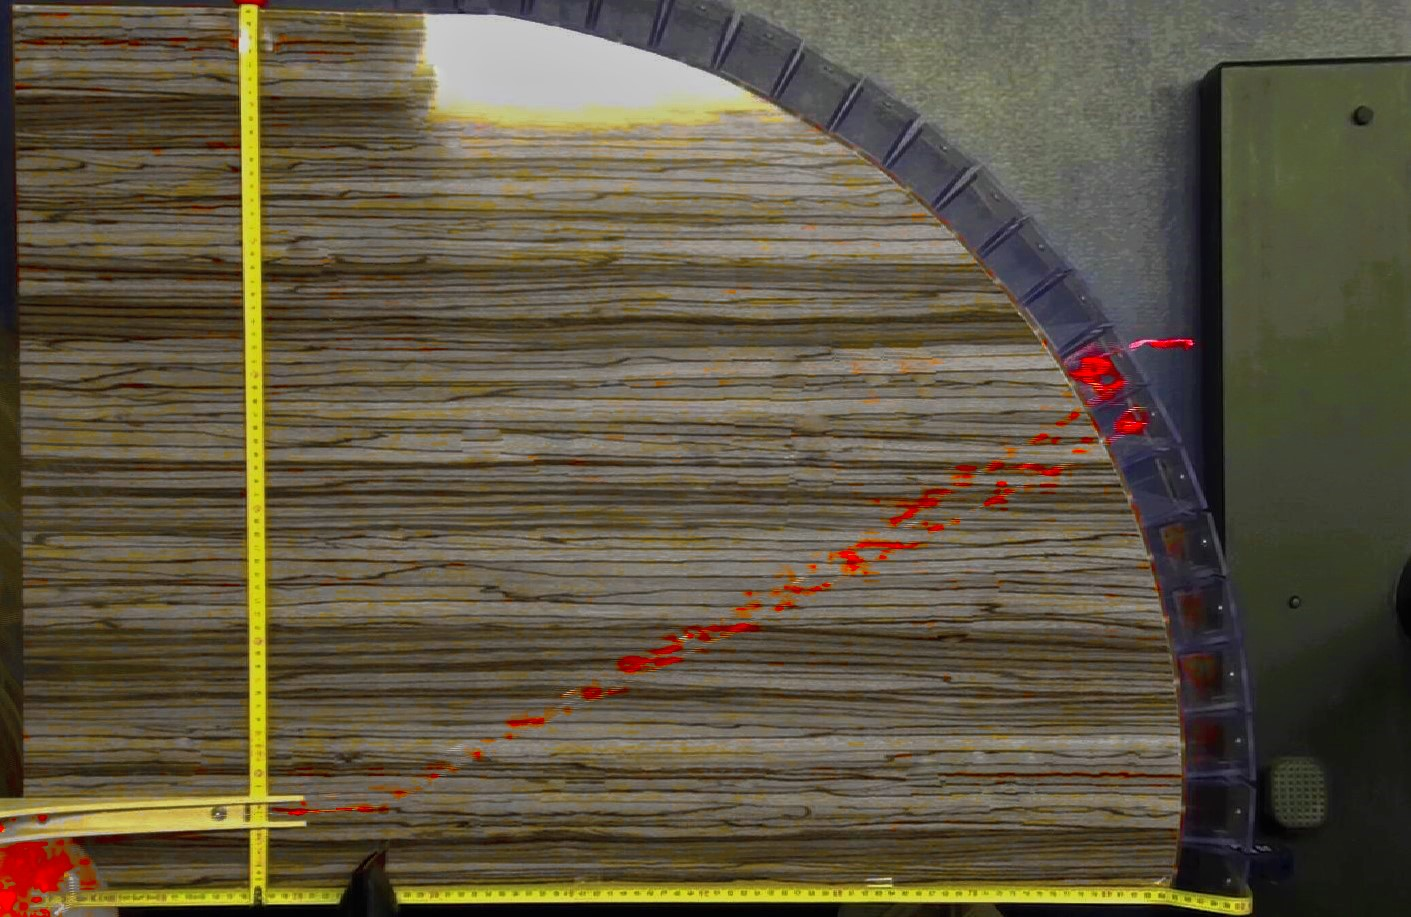
\includegraphics[width=0.99\textwidth]{images/strobe1.jpg}
  \caption[Exemplarische Stroboskopaufnahme der ersten Messreihe]{Exemplarisches Bildschirmfoto mit Stroboskopfilter der ersten Messreihe. Wegen des geringen Kontrastes zwischen den roten Kugeln und der bräunlichen Arbeitsplatte werden Farbfilter angewendet, um die Bahnkurven besser erkennbar zu machen. Bei der Auswertung einzelner Bilder in der Software \textit{Tracker} sind die Kugeln bis auf eine Bewegungsverzerrung gut erkennbar.}
  \label{fig:strobe1}
  \vspace{-0pt}
\end{figure}